% !TEX root = ../../main.tex


\begin{figure}[p]
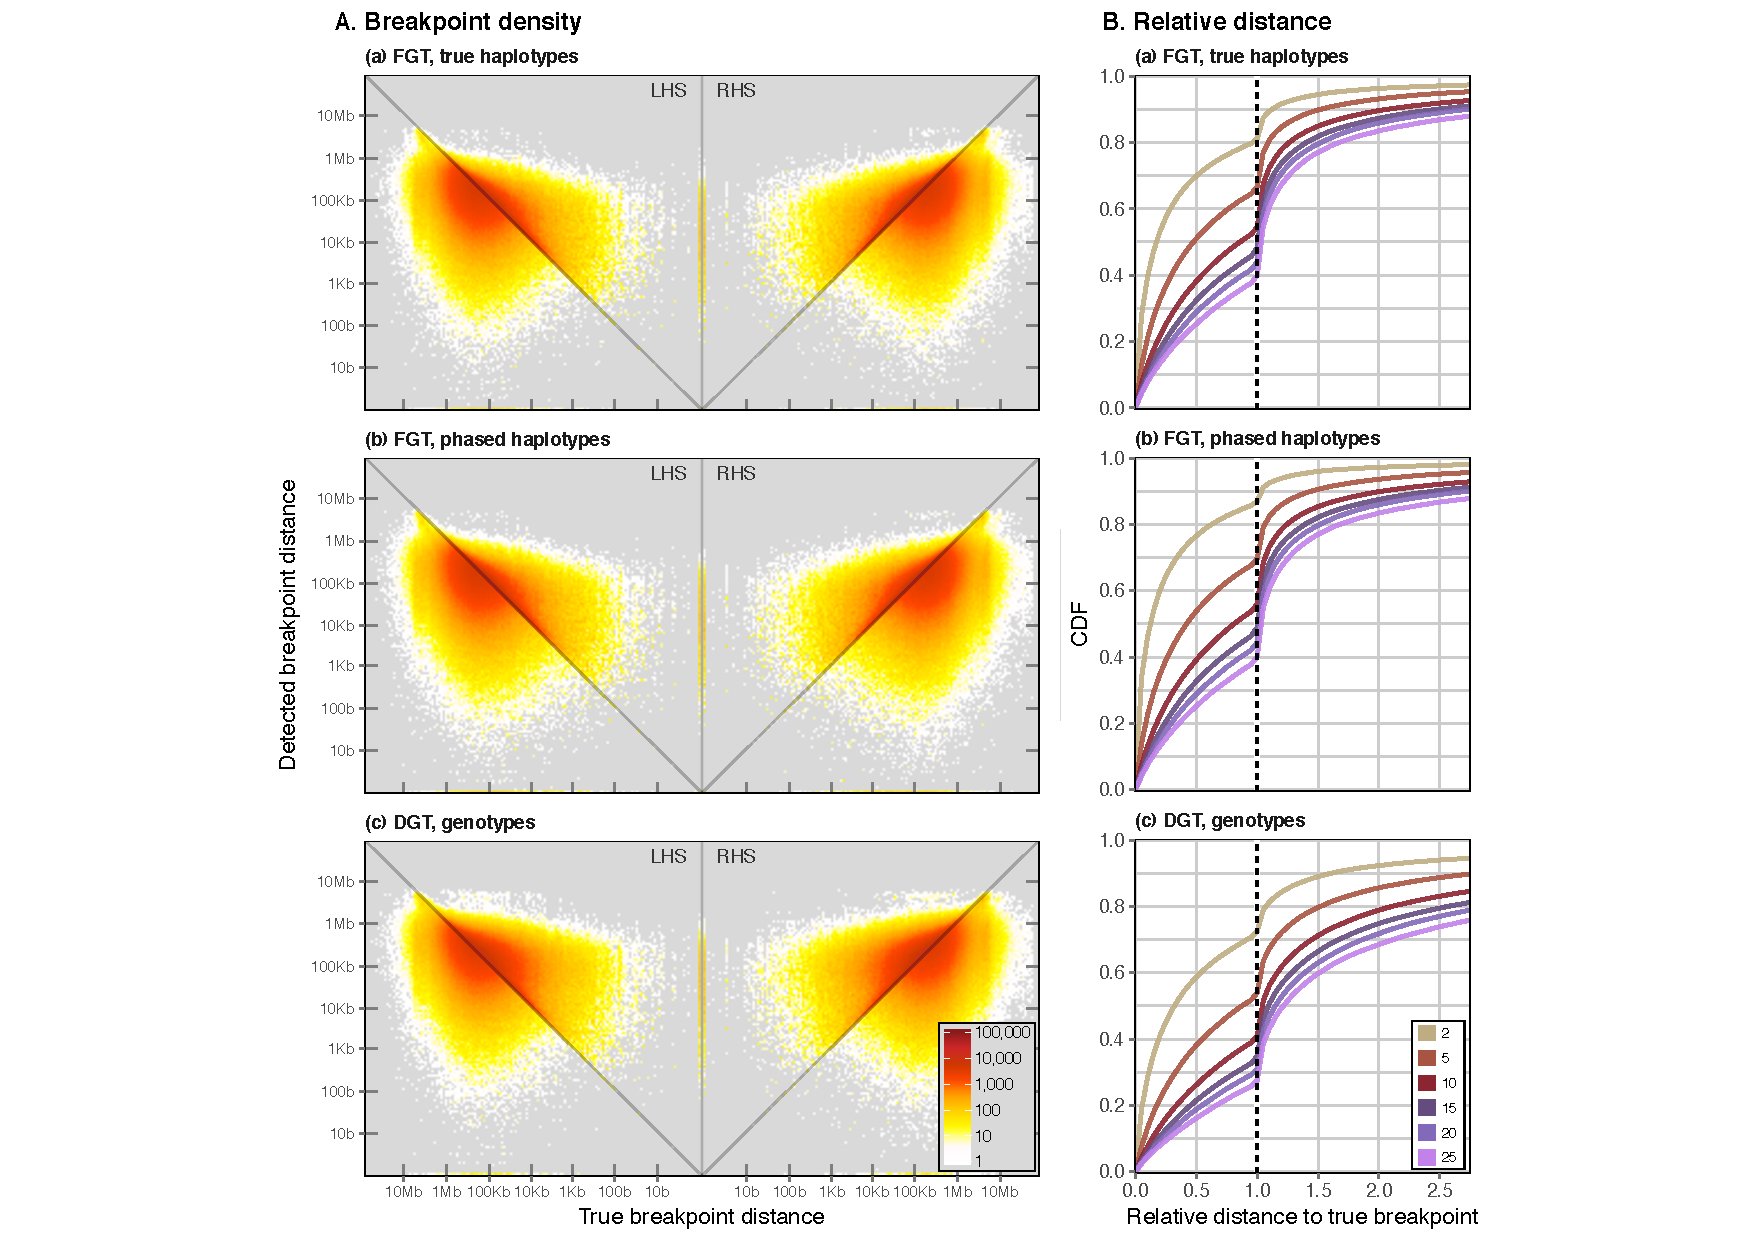
\includegraphics[width=\textwidth]{./img/ch4/break_naive_err}
\Caption{Accuracy of IBD detection using \emph{tidy} after inclusion of genotype error}
{Simulated data after the inclusion of error was analysed using the \gls{fgt} on true haplotypes (a), phased haplotypes (b), and the \gls{dgt} on genotype data (c).
Panel~\textbf{(A)} shows the density of true and detected breakpoints in terms of the physical distance between each detected breakpoint and the corresponding focal site; shown separately for breakpoints detected on the left (LHS) and right-hand side (RHS) of a focal position.
The number of detected and true breakpoints is indicated by colour intensity.
Panel~\textbf{(B)} shows the physical length in terms of the relative distance between a focal site and the detected breakpoint, $\hat{d}$, normalised by the distance to the true breakpoint, $d$; \ie relative distance was calculated as $\rfrac{\hat{d}}{d}$, such that $<1$ indicates underestimation and and $>1$ overestimation of detected breakpoint distance.
This is shown as the cumulative density per \fk{}~variant, for ${k \in \{2, 5, 10, 15, 20, 25\}}$.}
{fig:naive_break_err}
\end{figure}
